%%%%%%%%%% Commands --

%% General commands
\newcommand{\todo}[1]{\emph{\textcolor{red}{TODO: #1}}}
\newcommand{\note}[1]{\emph{\textcolor{blue}{NOTE: #1}}}
\newcommand{\panic}[1]{\textbf{\textcolor{red}{(#1)}}}

\renewcommand{\subsectionautorefname}{section}
\renewcommand{\subsubsectionautorefname}{section}

\newcommand{\ie}{i.e.,}
\newcommand{\eg}{e.g.,}
\newcommand{\aka}{a.k.a.}

\newcommand{\tuple}[1]{\langle #1 \rangle}
\renewcommand\qedsymbol{$\blacksquare$}

%% Hemiola

\newcommand{\hemiola}{Hemiola}

\newcommand{\listof}[1]{\ensuremath{\mathbf{#1}}}
\newcommand{\listtof}[1]{\ensuremath{\overrightarrow{#1}}}
\newcommand{\listnil}{\ensuremath{\lbrack\rbrack}}
\newcommand{\listcons}[2]{\ensuremath{#1 : #2}}
\newcommand{\listsingle}[1]{\ensuremath{\lbrack #1 \rbrack}}
\newcommand{\listapp}[2]{\ensuremath{#1 + #2}}
\newcommand{\listsub}[2]{\ensuremath{#1 - #2}}
\newcommand{\listdisj}[2]{\ensuremath{#1 \; \# \; #2}}
\newcommand{\listconcat}[1]{\ensuremath{\widehat{#1}}}
\newcommand{\sizeof}[1]{\ensuremath{|\, #1\, |}}

\newcommand{\mapupd}[3]{\listapp{#1}{(#2, #3)}}
\newcommand{\mapupds}[2]{\listapp{#1}{#2}}
\newcommand{\mapsubs}[2]{\listsub{#1}{#2}}

\newcommand{\idxOf}[1]{\ensuremath{#1.i}}

\newcommand{\propt}{\ensuremath{\mathbb{P}}}
\newcommand{\hidt}{\ensuremath{\mathbb{I}}}
\newcommand{\hvaluet}{\ensuremath{\mathbb{V}}}
\newcommand{\hmsgt}{\ensuremath{\mathbb{M}}}
\newcommand{\hostt}{\ensuremath{\mathbb{O}}}
\newcommand{\hsyst}{\ensuremath{\mathbb{S}}}
\newcommand{\hidmt}{\ensuremath{\hidt \ast \hmsgt}}
\newcommand{\hprect}{\ensuremath{\mathcal{P}}}
\newcommand{\htrst}{\ensuremath{\mathcal{T}}}

\newcommand{\hsysIn}[1]{\ensuremath{\listof{#1_{\textrm{in}}}}}
\newcommand{\hsysRq}[1]{\ensuremath{\listof{#1_{\textrm{rq}}}}}
\newcommand{\hsysRs}[1]{\ensuremath{\listof{#1_{\textrm{rs}}}}}
\newcommand{\hsys}[4]{\ensuremath{\tuple{#1, #2, #3, #4}}}
\newcommand{\hsyss}[2]{\hsys{#1}{\hsysIn{#2}}{\hsysRq{#2}}{\hsysRs{#2}}}
\newcommand{\hsysInA}[1]{\ensuremath{#1.\hsysIn{i}}}
\newcommand{\hsysRqA}[1]{\ensuremath{#1.\hsysRq{i}}}
\newcommand{\hsysRsA}[1]{\ensuremath{#1.\hsysRs{i}}}

\newcommand{\hsysobjs}[1]{\ensuremath{#1.\listof{O}}}
\newcommand{\hobjrules}[1]{\ensuremath{#1.\listof{r}}}

\newcommand{\msgIns}[1]{\listof{#1^{\textrm{ins}}}}
\newcommand{\msgOuts}[1]{\listof{#1^{\textrm{outs}}}}
\newcommand{\midxIns}[1]{\listof{\idxOf{#1^{\textrm{ins}}}}}
\newcommand{\midxOuts}[1]{\listof{\idxOf{#1^{\textrm{outs}}}}}

\newcommand{\lblEmpty}{\ensuremath{l_\epsilon}}
\newcommand{\lblIns}[1]{\ensuremath{l_{\textrm{in}}(#1)}}
\newcommand{\lblOuts}[1]{\ensuremath{l_{\textrm{out}}(#1)}}
\newcommand{\lblInt}[4]{\ensuremath{l_{\textrm{int}}(#1, #2, #3, #4)}}

\newcommand{\hmpt}{\ensuremath{\mathcal{M}}}
\newcommand{\hsttr}{\ensuremath{\listtof{\hostt} \ast \hmpt}}
\newcommand{\hstt}{\ensuremath{\mathbb{S}}}
\newcommand{\hst}[2]{\ensuremath{\tuple{#1, #2}}}
\newcommand{\hstm}[2]{\ensuremath{\left\langle\begin{array}{l}#1,\\ #2 \end{array}\right\rangle}}
\newcommand{\sysInit}[1]{\ensuremath{#1_{\textsf{init}}}}

\newcommand{\disj}[2]{\ensuremath{#1 \; \# \; #2}}
\newcommand{\nodup}[1]{\ensuremath{\textsf{nodup}\: #1}}

\newcommand{\semstep}[4]{\ensuremath{#2 \xrightarrow[#1]{#3} #4}}
\newcommand{\semsteps}[4]{\ensuremath{#2 \xRightarrow[#1]{#3} #4}}
\newcommand{\semrch}[2]{\ensuremath{#1 \Rightarrow #2}}
\newcommand{\semleg}[2]{\ensuremath{#1 \xRightarrow{#2} \bullet}}
\newcommand{\sembeh}[2]{\ensuremath{#1 \Downarrow #2}}
\newcommand{\behOf}[1]{\ensuremath{\widetilde{#1}}}

\newcommand{\refines}[2]{\ensuremath{#1 \sqsubseteq #2}}

\newcommand{\enqMsgs}[2]{\mapupds{#1}{#2}}
\newcommand{\deqMsgs}[2]{\mapsubs{#1}{#2}}

%% Serializability

\newcommand{\atomic}[3]{\ensuremath{#1 \stackrel{#2}{\rightsquigarrow} #3}}
\newcommand{\atomicLong}[3]{\ensuremath{#1 \frac{\scriptstyle{#2}}{}\hspace{-5pt}\rightsquigarrow #3}}
\newcommand{\extatomic}[4]{\ensuremath{#1 \vdash #2 \stackrel{#3}{\rightsquigarrow}_{\textsf{ext}} #4}}
\newcommand{\extatomicLong}[4]{\ensuremath{#1 \vdash #2 \frac{\scriptstyle{#3}}{}\hspace{-5pt}\rightsquigarrow_{\textsf{ext}} #4}}
\newcommand{\trsn}[2]{\ensuremath{#1 \sswarrow #2}}

\newcommand{\extatomicshort}[2]{\ensuremath{#1 \stackrel{#2}{\rightsquigarrow}_{\textsf{ext}}}}
\newcommand{\intatomicshort}[2]{\ensuremath{#1 \stackrel{#2}{\rightsquigarrow}_{\textsf{int}}}}

\newcommand{\amsgi}[1]{\ensuremath{#1^{\textrm{init}}}}
\newcommand{\amsge}[1]{\ensuremath{#1^{\textrm{end}}}}

\newcommand{\hseq}[2]{\ensuremath{#1 \parallel #2}}
\newcommand{\hsrzl}[2]{\ensuremath{\mathit{Serializable}\ #1\ #2}}
\newcommand{\hsrz}[1]{\ensuremath{\mathit{Serializable}\ #1}}

\newcommand{\strsn}[2]{\ensuremath{#1 \sswarrow_{s} #2}}
\newcommand{\hsseq}[3]{\ensuremath{#1 \parallel_{#3} #2}}

%%%%%%%%%% Contents --

\section{Introduction}\label{sec-intro}

Cache-coherence protocols have been regarded as one of the greatest correctness challenges of the hardware world.
Industry has most commonly used testing and bounded model checking for quality assurance of cache-coherence implementations, but these techniques are not sound and sometimes miss subtle bugs~\cite{ccbug}.

Research on model checking and theorem proving has produced sound techniques, though typically with significant limitations:
either the verification is of a specific protocol, or state-space-explosion concerns limit applicability to quite small cache topologies~\cite{Komuravelli:2014,Murali:2015,Banks:2017,Oswald:2018}.
In order to overcome the latter, recent approaches~\cite{Chen:2008,Chen:2010,McMillan:2016,Opeoluwa:2016,Opeoluwa:2017,Oswald:2020} utilized the notion of \emph{modularity} and successfully built verification tools that are scalable enough to verify hierarchical cache-coherence protocols.

However, these modularity disciplines impose significant restrictions in protocol design, in order to obtain clear module boundaries among caches.
A concrete limitation of modular design and verification comes when trying to verify cache-coherence protocols that are not \emph{inclusive}.
Noninclusive caches have been in common industrial use for a decade: AMD Opteron servers are known to use exclusive caches~\cite{Irazoqui:2016}, and Intel Skylake-X processors use noninclusive\footnote{Intel uses the term ``noninclusive cache'' to say that the cache is neither inclusive nor exclusive.} caches~\cite{intel-non-inclusive,Zhao:2010,Yan:2019}.

I would like to view the verification of hierarchical cache-coherence protocols from a different perspective.
Instead of decomposing a protocol design and proof, we view a cache-coherence protocol as a \emph{global} distributed protocol and look for commonalities across well-designed protocols.
It is a good start to identify ``good-hygiene'' properties, but it is even better to formalize such properties in frameworks that guide the design of protocols.
Then we can provide nonobvious and useful reasoning principles by-construction.

Looking for another way to factor proofs, we can find a hint in terminology often employed by protocol designers and verification engineers.
These protocols are distributed message-passing systems, so we can apply traditional software terminology like \emph{transaction} to them directly, and in fact we find similar intuitions employed in practice.
In order to describe a case where the protocol deals with two different requests passing through the same cache, for instance, a designer often says ``this cache acts like a \emph{serialization point} so the two transactions can safely \emph{interleave} with each other.''
While the notions of interleaving and serialization are already pervasive, I have found no past work trying to find a minimal set of conditions that ensure transactions are always serialized, formalizing them in a reusable framework.

In this proposal, I propose a framework called \hemiola{}, embedded in the Coq proof assistant, which dramatically decreases the burden of designing and formally proving hierarchical cache-coherence protocols.
In particular, on top of the framework, hardware developers can design cache-coherence protocols without worrying about possible complex interleavings among different transactions, standing for different concurrent memory accesses.
From the verification perspective, it is established that any invariant of a protocol under serialized execution is also an invariant under the interleaved executions that are necessary for good performance.

More specifically, \hemiola{} formalizes a set of message-passing distributed protocols with tree hierarchies and particular topologies of channels between nodes, with associated locks.
These protocols are defined by associating each tree node with a set of local state-transition rules that may remove messages from incoming queues and add messages to outgoing queues.
\hemiola{} exposes a domain-specific language of protocols, such that any expressible program is guaranteed to validate a \emph{serializability} property for single memory requests.
Furthermore, the framework provides a novel invariant proof method that only requires consideration of execution histories that do not interleave memory accesses -- so that almost all formal reasoning about concurrency is confined to the framework, not proofs of individual protocols.

To demonstrate usability of the framework, I plan to provide complete correctness proofs of hierarchical, noninclusive cache-coherence protocols as case studies.
A compilation/synthesis toolchain will also be provided, which converts a cache-coherence protocol described in \hemiola{} to a corresponding hardware implementation running on FPGAs.
A so-called protocol compiler would take such a role, which employes predesigned, optimized hardware components such as caches and resource controllers.

\section{Motivation and Background}

\subsection{Challenges in designing cache-coherence protocols}

Before proposing the \hemiola{} framework, we provide a simple yet motivating example to introduce cache-coherence protocols and typical challenges in the design and verification.
For simplicity, in this section, we will consider only \emph{a single memory location} and design a protocol only for this location.
We will see it is still nontrivial to design a correct protocol.

\tikzset{
  msi/.pic = {
    \node at (0, 0) {$P(S, v, S_{\tuple{1, 2}})$};
    \node at (-1.5, -1.5) {$C_1(S, v)$};
    \node at (1.5, -1.5) {$C_2(S, v)$};
    % between P and C_1
    \draw [<-<] (-0.6, -0.3) -- (-1.5, -1.2);
    \draw [<-<] (-0.4, -0.3) -- (-1.3, -1.2);
    \draw [>->] (-0.2, -0.3) -- (-1.1, -1.2);
    % between P and C_2
    \draw [<-<] (0.6, -0.3) -- (1.5, -1.2);
    \draw [<-<] (0.4, -0.3) -- (1.3, -1.2);
    \draw [>->] (0.2, -0.3) -- (1.1, -1.2);
    % C_1 external
    \draw [<-<] (-1.6, -1.8) -- (-1.6, -2.3);
    \draw [>->] (-1.4, -1.8) -- (-1.4, -2.3);
    % C_2 external
    \draw [<-<] (1.6, -1.8) -- (1.6, -2.3);
    \draw [>->] (1.4, -1.8) -- (1.4, -2.3);
  },
  msipc1/.pic = {
    \node at (0, 0) {$P(S, v, S_{\tuple{1, 2}})$};
    \node at (0, -1.5) {$C_1(S, v)$};
    % between P and C_1
    \draw [<-<] (-0.2, -0.3) -- (-0.2, -1.2);
    \draw [<-<] (0, -0.3) -- (0, -1.2);
    \draw [>->] (0.2, -0.3) -- (0.2, -1.2);
    % C_1 external
    \draw [<-<] (-0.1, -1.8) -- (-0.1, -2.3);
    \draw [>->] (0.1, -1.8) -- (0.1, -2.3);
  },
  msipc2/.pic = {
    \node at (0, 0) {$P(S, v, S_{\tuple{1, 2}})$};
    \node at (0, -1.5) {$C_2(I, \cdot)$};
    % between P and C_1
    \draw [<-<] (-0.4, -0.3) -- (-0.4, -1.2);
    \draw [<-<] (-0.2, -0.3) -- (-0.2, -1.2);
    \draw [>->] (0.4, -0.3) -- (0.4, -1.2);
    % C_1 external
    \draw [<-<] (-0.1, -1.8) -- (-0.1, -2.3);
    \draw [>->] (0.1, -1.8) -- (0.1, -2.3);
  },
  msipc3/.pic = {
    \node at (0, 0) {$P(I, \cdot, M_{\tuple{1}})$};
    \node at (0, -1.5) {$C_1(S, v)$};
    \node at (1.8, 0) {$C_2(I, \cdot)$};
    % between P and C_1
    \draw [<-<] (-0.2, -0.3) -- (-0.2, -1.2);
    \draw [<-<] (0, -0.3) -- (0, -1.2);
    \draw [>->] (0.2, -0.3) -- (0.2, -1.2);
    % between P and C_2
    \draw [<->] (0.9, 0) -- (1.2, 0);
    % C_1 external
    \draw [<-<] (-0.1, -1.8) -- (-0.1, -2.3);
    \draw [>->] (0.1, -1.8) -- (0.1, -2.3);
  },
  spec/.pic = {
    \node at (0, 0) {$\textrm{Spec}(v)$};
    % C_1 external
    \draw [<-<] (-0.4, -0.3) -- (-0.5, -0.8);
    \draw [>->] (-0.2, -0.3) -- (-0.3, -0.8);
    % C_2 external
    \draw [<-<] (0.4, -0.3) -- (0.5, -0.8);
    \draw [>->] (0.2, -0.3) -- (0.3, -0.8);
  }
}
\begin{figure}[h]
  \centering
  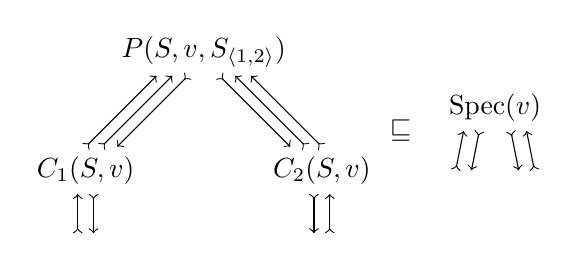
\begin{tikzpicture}
    \pic at (0, 0) {msi};
    \node at (2.5, -1) {$\sqsubseteq$};
    \pic at (3.7, -0.7) {spec};
  \end{tikzpicture}
  \caption{A simple MSI directory protocol}
  \vspace{-5pt}
  \label{fig-motive-1}
\end{figure}

The overall goal of cache coherence is, as the name suggests, to preserve coherence among multiple candidate values in a memory subsystem.
In other words, if the system is coherent, then it should behave like an ordinary memory.
\autoref{fig-motive-1} shows objects and channels for a simple directory-based MSI protocol.
Since we deal with only a single memory location, the specification (RHS of $\sqsubseteq$) is a single-value ($v$) container with atomic read and write.

Looking at the implementation (LHS of $\sqsubseteq$), there are three objects $P$, $C_1$, and $C_2$, and each of them has its own status (M, S, or I) and data ($v$).
A status of an object represents a permission on its local replica.
In this MSI protocol, an object can read/write the data with the M (``modified'') status, only read with S (``shared''), and cannot read/write with I (``invalid'').
The parent $P$ additionally has a data structure called a \emph{directory} to track the statuses of the children.
For example, a directory might be $S_{\tuple{1, 2}}$, meaning that both $C_1$ and $C_2$ have S status, in some logical snapshot of state.

Objects communicate through ordered channels (shown as $\rightarrowtail$ in the figure).
$C_1$ and $C_2$ have channels to receive and respond to external requests (from processor cores).
There are three types of channels between a parent and a child: a single channel for parent-to-child messages and two channels for child-to-parent requests and responses, respectively.
It is natural to wonder why two separate channels are required from a child to a parent; we will see the reason very soon.
Note that channels are depicted in a logical way; the actual hardware implementation may use different hardware components (\eg{} finite-capacity FIFOs or buses) that can simulate ordered channels.

\newcommand{\blackdiamond}{\raisebox{.4ex}{\ensuremath{\scriptscriptstyle\blacklozenge}}}
\begin{figure}[h]
  \centering
  \begin{subfigure}[b]{0.30\columnwidth}
    \centering
    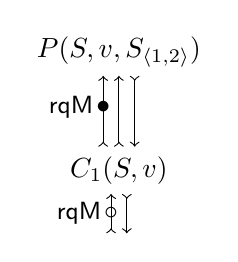
\begin{tikzpicture}
      \pic at (0, 0) {msipc1};
      \node[label={[label distance=-6pt]left:{\small {\sf rqM}}}] at (-0.2, -0.7) {$\bullet$};
      \node[label={[label distance=-6pt]left:{\small {\sf rqM}}}] at (-0.1, -2.05) {$\circ$};
    \end{tikzpicture}
    \caption{$C_1$ requesting to the parent}
    \label{fig-motive-2-a}
  \end{subfigure}
  \begin{subfigure}[b]{0.36\columnwidth}
    \centering
    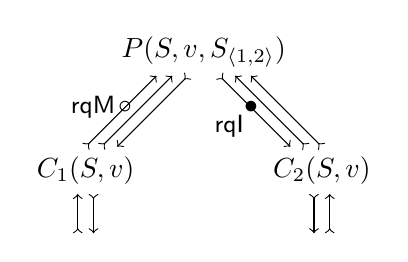
\begin{tikzpicture}
      \pic at (0, 0) {msi};
      \node[label={[label distance=-6pt]left:{\small {\sf rqM}}}] at (-1, -0.7) {$\circ$};
      \node[label={[label distance=-8pt]210:{\small {\sf rqI}}}] at (0.6, -0.7) {$\bullet$};
    \end{tikzpicture}
    \caption{$P$ making an invalidation request}
    \label{fig-motive-2-b}
  \end{subfigure}
  \begin{subfigure}[b]{0.30\columnwidth}
    \centering
    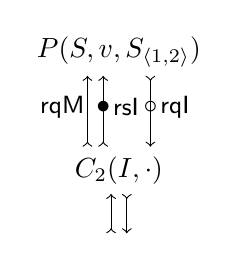
\begin{tikzpicture}
      \pic at (0, 0) {msipc2};
      \node[label={[label distance=-6pt]left:{\small {\sf rqM}}}] at (-0.4, -0.7) {$\blackdiamond$};
      \node[label={[label distance=-6pt]right:{\small {\sf rqI}}}] at (0.4, -0.7) {$\circ$};
      \node[label={[label distance=-6pt]right:{\small {\sf rsI}}}] at (-0.2, -0.7) {$\bullet$};
    \end{tikzpicture}
    \caption{$C_2$ responding to the parent}
    \label{fig-motive-2-c}
  \end{subfigure}
  \caption{Rule-execution cases in the simple MSI protocol}
  \vspace{-5pt}
  \label{fig-motive-2}
\end{figure}

All objects run concurrently, repeatedly executing \emph{rules} that define local state transitions.
In message-passing systems, a rule may take some messages from input channels, perform a state transition, and put messages in output channels.
A rule may also have a precondition, blocking use of that rule when the precondition does not hold.
\autoref{fig-motive-2} shows some example rule-execution cases depending on statuses of the objects.
\autoref{fig-motive-2-a} is the case where a child $C_1$ takes an external request ($\textsf{rqM}\circ$) to write data, but it does not have M status and thus forwards the request to the parent ($\textsf{rqM}\bullet$).
At this moment the child usually \emph{sets a lock} not to allow any further external requests for the value.
The following pseudocode describes the rule:
\begin{lstlisting}
Rule c1RqMToP :=
  assert !C1.locked();
  assert (C1.status != M);
  assert (C1.extRq.first == rqM);
  C1.extRq.deq();
  C1.rqToP.enq(rqM);
  C1.lock();
Endrule
\end{lstlisting}
The rule checks whether $C_1$ is not locked so it can handle $\textsf{rqM}\circ$, confirms it does not have a write permission, dequeues an external request from \slstinline{extRq}, sends a request to $P$ by using a channel \slstinline{rqToP}, and sets a lock.

As a next rule-execution step, $\textsf{rqM}\circ$ (previously outputted from \autoref{fig-motive-2-a}) is handled by the parent $P$, as shown in \autoref{fig-motive-2-b}.
It makes \emph{invalidation} requests ($\textsf{rqI}$) to the other children ($C_2$ is the only other child in this system) to change their statuses to I, since when a child has M the others should not be able to read/write the data.
After making invalidation requests, the parent also sets a lock to disallow requests from the children.

Now imagine a scenario where two children $C_1$ and $C_2$ requested $\textsf{rqM}$ to the parent (to obtain M) at the same time, and the parent decided to deal with the request from $C_1$ first.
Proper locking is indeed required here, since otherwise the parent will handle two $\textsf{rqM}$s simultaneously, which might lead to an incoherent state -- two M statuses in the system.
\autoref{fig-motive-2-c} presents this case, where an invalidation request was made to $C_2$ ($\textsf{rqI}\circ$) and even before this, $C_2$ requested $\textsf{rqM}\blackdiamond$ to the parent.
In order to handle all the requests correctly, we should carefully consider some corner cases:
\begin{itemize}
\item Since $C_2$ requested $\textsf{rqM}\blackdiamond$, it is locked when the $\textsf{rqI}\circ$ message arrives. It should still be able to handle this invalidation request even if it is locked. We see that \emph{locking should be fine-grained enough to distinguish message kinds} while handling a request.
\item Due to the existence of $\textsf{rqM}\blackdiamond$, if we had a single channel from a child to a parent, a deadlock would occur. $P$ cannot take $\textsf{rqM}\blackdiamond$ since it was locked after making an invalidation request. It cannot take $\textsf{rsI}\bullet$ as well since the response is not the first one of the ordered channel. This case shows the necessity of having multiple channels between a child and a parent.
\end{itemize}

A so-called three-channel system has been widely used and regarded as a good choice to make the design correct and live~\cite{Murali:2015,thesis:Murali:2016}.
While there are other possible correct topology and network settings, the cases shown in \autoref{fig-motive-2} at least demonstrate that it is nontrivial to construct one of them.

If proper topology and locking are crucial for designing a correct protocol, can we craft a domain-specific language where only conformant protocols are expressible?
That is exactly what we plan to reflect in \hemiola{}, where, for instance, instead of the above pseudocode, rules are written more like the following one:
\begin{lstlisting}
Rule c1RqMToP :=
  using template RqToP;
  accepts rqM;
  assert (me.status != M);
  release rqM;
Endrule
\end{lstlisting}
Note that this pseudocode does not mention specific channels or locking at all.
Instead, it just says that the rule is for making a request to the parent (\slstinline{RqToP}), and it gives various associated assertions and actions, fitting slots associated with this kind of rule.

\hemiola{} provides \emph{rule templates} that employ proven-safe topologies and network structures and automatically set associated locks, so designers can design protocols without worrying about corner cases due to interleavings.

We further discovered that if a system is defined by using these rule templates, global invariants can be proven without explicit consideration of interference by concurrently executing memory accesses.
The key is the notion of \emph{serializability} coming originally from the database-transactions literature.

\subsection{Serializability in distributed systems}

\subsubsection{Baseline: protocol transition systems}
\label{sec-trs}

\paragraph{Notations.}
Throughout this proposal, we will use several notations for lists (sequences) and finite maps.
A bold character (\eg{} $\listof{l}$) denotes a list.
$\listnil{}$, $(\listcons{h}{\listof{t}})$, $(\listapp{\listof{l_1}}{\listof{l_2}})$, $(\listsub{\listof{l_1}}{\listof{l_2}})$, and
$(\listdisj{\listof{l_1}}{\listof{l_2}})$ denote nil, cons, append, subtraction, and disjointness of lists, respectively.
$\listconcat{\listof{l}}$ flattens the list of lists $\listof{l}$ with repeated concatenation.
$\sizeof{\listof{l}}$ is the length of a list.
Regarding a list of key-value pairs as a finite map, we override notations for lists.
For example, $(\mapupds{M}{\listof{l}})$ updates multiple key-value pairs in a finite map $M$.
Moreover, we overload the same operation $(\mapupd{M}{k}{v})$ for a single update for simplicity.

\paragraph{Syntax.}

\begin{figure}[h]
  \centering\small
  \begin{tabular}{|c|c|}
    \hline
    \begin{math}
      \begin{array}{rl}
        \textrm{Index} & i \in \hidt{} \\
        \textrm{Value} & v \in \hvaluet{} \\
        \textrm{Message} & m ::= \tuple{i, v} \in \hmsgt{} \triangleq \hidt \ast \hvaluet \\
        \textrm{Object state} & o \in \hostt{} \\
        \textrm{Rule precondition} & p \in
        \hprect \triangleq \hostt \to \listtof{\hidmt} \to \propt \\
        \textrm{Rule transition} & t \in
        \htrst \triangleq \hostt \to \listtof{\hidmt} \to \hostt \ast \listtof{\hidmt} \\
      \end{array}
    \end{math} &
    \begin{math}
      \begin{array}{rl}
        \textrm{Rule} & r ::= \tuple{i, p, t} \\
        \textrm{Object} & O ::= \tuple{i, \listof{r}} \\
        \textrm{System} & S ::= \hsyss{\listof{O}}{i} \\
      \end{array}
    \end{math}\\
    \hline
  \end{tabular}
  \caption{Protocol transition system}
  \label{fig-trs-system}
\end{figure}

We first formally define protocol transition systems, which will be an underlying basis for the domain-specific language in \hemiola{}.
\autoref{fig-trs-system} explains what such systems are, in the style of automata theory.
Our definition is shallowly embedded in Coq, \eg{} precondition and transition definitions use native Coq function types.
A struct (a rule, an object, etc.)  sometimes has an \emph{index} to distinguish it from the other components.
We will use $\tuple{\cdot}$ to denote a struct and use a name to access a field value.
In our implementation, an index is a list of natural numbers, for easy hierarchical addressing.
A \emph{value} $v$ refers to a general set of values, principally those that can be stored at memory addresses.
A \emph{message} $m$ consists of a message id (effectively from an enumeration of message kinds) and value.

A system $S$ contains information about objects and channels.
It consists of objects (\listof{O}) and channel indices for internal messages (\hsysIn{i}), external inputs (\hsysRq{i}), and external outputs (\hsysRs{i}).
Each object (or channel) has its own unique index.
The definition is general in that any object can access any channel in the system, just by mentioning the channel index in a state transition.
It is necessary to distinguish between internal and external channels, in order to define external behaviors of the system.
An object $O$ contains its object index (unique within a system) and rules (\listof{r}) that make local state transitions within the object.

A rule $r$ consists of its rule index (unique within an object), a precondition ($p$), and a transition function ($t$).
A precondition takes two arguments, a current object state and a list of (channel index, message) pairs as input messages, and decides whether the rule can be executed or not.
A transition function takes the same arguments but returns the next object state and a list of (channel index, message) pairs as output messages.

\begin{figure*}[t]
  \centering
  \begin{tabular}{|c|}
    \hline
    \begin{math}
      \begin{array}{c}
        \inference[StepSilent:]{}{\semstep{S}{s}{\lblEmpty{}}{s}} \\
        \mbox{}\vspace{-5pt} \\ %% padding
        \inference[StepIns:]{\listof{m} \neq \listnil
          & \listof{\idxOf{m}} \subseteq \hsysRqA{S}
          & \nodup{\listof{\idxOf{m}}}}{\semstep{S}
          {\hst{\listof{o}}{M}}
          {\lblIns{\listof{m}}}
          {\hst{\listof{o}}{\enqMsgs{M}{\listof{m}}}}} \\
        \mbox{}\vspace{-5pt} \\ %% padding
        \inference[StepOuts:]{\listof{m} \neq \listnil
          & \listof{\idxOf{m}} \subseteq \hsysRsA{S}
          & \nodup{\listof{\idxOf{m}}}}{\semstep{S}
          {\hst{\listof{o}}{M}}
          {\lblOuts{\listof{m}}}
          {\hst{\listof{o}}{\deqMsgs{M}{\listof{m}}}}} \\
        \mbox{}\vspace{-5pt} \\ %% padding
        \inference[StepInt:]{S = \hsyss{\listof{O}}{i}
          & O \in S.\listof{O}
          & r \in O.\listof{r} \\
          \midxIns{m} \subseteq \hsysInA{S} \cup \hsysRqA{S}
          & \nodup{\midxIns{m}} \\
          \listof{o}\ \idxOf{O} = o_0
          & r.p\ o_0\ \msgIns{m}
          & r.t\ o_0\ \msgIns{m} = (o_1, \msgOuts{m}) \\
          \midxOuts{m} \subseteq \hsysInA{S} \cup \hsysRsA{S}
          & \nodup{\midxOuts{m}}
          & \disj{\midxIns{m}}{\midxOuts{m}}}{\semstep{S}
          {\hst{\listof{o}}{M}}
          {\lblInt{\idxOf{O}}{\idxOf{r}}{\msgIns{m}}{\msgOuts{m}}}
          {\hstm{\mapupd{\listof{o}}{\idxOf{O}}{o_1}}{\enqMsgs{\deqMsgs{M}{\msgIns{m}}}{\msgOuts{m}}}}} \\
        \mbox{}\vspace{-5pt} \\ %% padding
      \end{array}
    \end{math}\\
    \hline
    \begin{math}
      \begin{array}{ccc}
        \mbox{}\vspace{-5pt} \\ %% padding
        \inference[StepsNil:]{}{\semsteps{S}{s}{\listnil{}}{s}} &
        \inference[StepsCons:]{\semsteps{S}{s_0}{\listof{l}}{s_1}
          & \semstep{S}{s_1}{l_1}{s_2}}{\semsteps{S}{s_0}{\listcons{l_1}{\listof{l}}}{s_2}} &
        \inference[Behavior:]{\semsteps{S}{\sysInit{S}}{\listof{l}}{s}}{\sembeh{S}{\behOf{\listof{l}}}} \\
        \mbox{}\vspace{-5pt} \\ %% padding
      \end{array}
    \end{math}\\
    \hline
  \end{tabular}
  \caption{Semantics of protocol transition systems}
  \vspace{-10pt}
  \label{fig-trs-semantics}
\end{figure*}

\paragraph{Semantics.}
\autoref{fig-trs-semantics} describes the semantics of protocol transition systems.
A state transition (step) happens by a rule that takes input messages and generates output messages.
The semantics for a step is presented as a judgment $\semstep{S}{s_0}{l}{s_1}$, where $S$ is the system to execute, $s_0$ is a prestate, $s_1$ is a poststate, and $l$ is a label generated by the state transition.
The state of a system (in domain $\hsyst{}$) is a pair, consisting of object states and message states.
Object states are represented in finite maps from object indices to object states, and message states are represented in finite maps from channel indices to queues of messages.

Rule [StepSilent] represents the case where no state transition happens in the current step; an empty label (\lblEmpty{}) is generated in this case.
A system may accept input messages from the external world; [StepIns] describes this case, where the external input messages (\listof{m}) should not be empty, channels of the messages are valid, and none of them share the same channel ($\nodup{\listof{\idxOf{m}}}$); an external inputs label $(\lblIns{\listof{m}})$ is generated in this case.
[StepOuts] describes the opposite case, for output messages being released to the external world.

Lastly, [StepInt] deals with a state transition by a rule ($r$) in an object ($O$).
It nondeterministically chooses an object and a rule in the object, checks that the precondition holds, and applies the transition to update the state of the system; an internal label ($\lblInt{\idxOf{O}}{\idxOf{r}}{\msgIns{m}}{\msgOuts{m}}$) is generated in this case, which records an object index, a rule index, input messages, and output messages.

Note that the semantics is based on ordered channels, so messages are \emph{enqueued} and \emph{dequeued} in each state-transition case.
We use notations $\enqMsgs{M}{\listof{m}}$ and $\deqMsgs{M}{\listof{m}}$ for such operations, and especially when messages are dequeued we implicitly assume that each element in $\listof{m}$ is at the front of its queue.
It is also required that any state transition does not both dequeue and enqueue an element from the same queue; $\disj{\midxIns{m}}{\midxOuts{m}}$ in [StepInt] exactly describes this condition.

The step semantics is naturally lifted to one for multiple steps, presented as a judgment $\semsteps{S}{s_0}{\listof{l}}{s_1}$, where $S$, $s_0$, and $s_1$ are similar to ones in the step semantics, and $\listof{l}$ is a sequence of labels generated by executions of the steps.
[StepsNil] serves the case where no state transitions happen at all.
[StepsCons] is a natural inductive constructor that combines previous steps and a new one.
Note that the latest label is added to the head, thus the last label in the sequence is the oldest one.
(We found this convention convenient in Coq for usual reasons of functional-programming naturalness, and we stick with it in the paper version of the formalism to avoid transcription errors.)

We will sometimes call a sequence of labels a \emph{history}.
We say that a state $s$ is \emph{reachable} iff there is a history $\listof{l}$ such that $\semsteps{S}{\sysInit{S}}{\listof{l}}{s}$ holds.
We use a simpler notation $\semrch{S}{s}$ for reachable states.
We also apply the symmetrical notion that a history $\listof{l}$ is \emph{legal} iff there is a state $s$ such that $\semsteps{S}{\sysInit{S}}{\listof{l}}{s}$ holds.
We write $\semleg{S}{\listof{l}}$ to assert that a history is legal.

\paragraph{Behaviors and correctness.}
A system $S$ has a behavior $\behOf{\listof{l}}$ if there exists an execution of steps that generates $\listof{l}$, starting with the initial state of $S$ ([Behavior]).
Here the $\behOf{\cdot}$ operation filters out silent ($l_\epsilon$) and internal ($l_{\textrm{int}}$) labels so only the external parts remain.
We call such a sequence of labels a \emph{trace}.
Finally we define a notion of correctness in \hemiola{}.

\begin{definition}[Trace Refinement]
  A system $I$ (``implementation'') is said to trace-refine another system $S$
  (``specification''), written as $\refines{I}{S}$, iff every trace of $I$ is
  also a trace of $S$:
  \begin{displaymath}
    \refines{I}{S} \triangleq \forall \listof{t}.\; \sembeh{I}{\listof{t}} \to \sembeh{S}{\listof{t}}.
  \end{displaymath}
\end{definition}

\subsubsection{Serializability in protocol transition systems}

Serializability~\cite{sz1,sz2} is a celebrated notion of concurrency correctness that originated with databases and distributed systems.
While each transaction in a system affects multiple values, serializability guarantees that concurrent execution of such transactions is correct in that the effect (state change) is the same as if the transactions were executed serially, \ie{} atomically in some order with no interleaving.
The protocol transition system described in \autoref{sec-trs} follows standard ideas of message-passing systems, thus it is natural to define and reason about serializability.

\begin{figure}[t]
  \centering
  \begin{tabular}{|c|}
    \hline
    \begin{math}
      \arraycolsep=-2pt
      \begin{array}{c}
        \inference[AtomicStart:]{}{\atomicLong{\listof{\amsgi{m}}}{\listsingle{\lblInt{\idxOf{O}}{\idxOf{r}}{\listof{\amsgi{m}}}{\listof{\amsge{m}}}}}{\listof{\amsge{m}}}} \\
        \inference[AtomicCont:]{\atomic{\listof{\amsgi{m}}}{\listof{l}}{\listof{\amsge{m}}}
          & \msgIns{n} \neq \listnil
          & \msgIns{n} \subseteq \listof{\amsge{m}}}{\atomicLong{\listof{m_0}}{\listcons{\lblInt{\idxOf{O}}{\idxOf{r}}{\msgIns{n}}{\msgOuts{n}}}{\listof{l}}}{(\listapp{\listsub{\listof{\amsge{m}}}{\msgIns{n}}}{\msgOuts{n}}})} \\
        \mbox{}\vspace{-5pt} %% padding
      \end{array}
    \end{math}\\
    \hline
    \begin{math}
      \begin{array}{cc}
        \begin{array}{c}
          \inference[TrsSilent:]{}{\trsn{S}{\listsingle{\lblEmpty{}}}} \\
          \inference[TrsIns:]{}{\trsn{S}{\listsingle{\lblIns{\listof{m}}}}} \\
          \inference[TrsOuts:]{}{\trsn{S}{\listsingle{\lblOuts{\listof{m}}}}} \\
          \mbox{}\vspace{-5pt} %% padding
        \end{array} &
        \begin{array}{l}
          \textrm{\footnotesize TrsAtomic:} \\
          \inference[]{\extatomic{S}{\listof{\amsgi{m}}}{\listof{l}}{\listof{\amsge{m}}}}{\trsn{S}{\listof{l}}}
        \end{array} \\
      \end{array}
    \end{math}\\
    \hline
  \end{tabular}
  \caption{Atomic histories and transactions}
  \vspace{-5pt}
  \label{fig-hemiola-trs}
\end{figure}

\paragraph{Atomic histories.}
In order to define serializability formally, we first provide basic definitions of atomic histories and transactions, in \autoref{fig-hemiola-trs}.
A history $h$ is \emph{atomic} iff it satisfies the predicate $(\atomic{\listof{\amsgi{m}}}{h}{\listof{\amsge{m}}})$ with \emph{starting messages} $\listof{\amsgi{m}}$ and \emph{live messages} $\listof{\amsge{m}}$.
[AtomicStart] initializes a history with an internal label for its first step.
[AtomicCont] inductively adds a label to an atomic history, where the input messages of the new label should be from live messages of the previous atomic history.

\begin{figure}[h]
  \centering
  \begin{tabular}{c}
    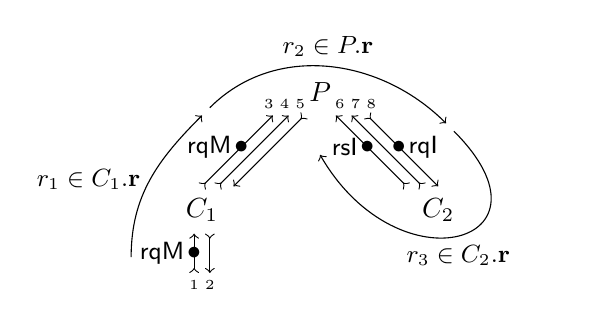
\begin{tikzpicture}
      \node at (0, 0) {$P$};
      \node at (-1.5, -1.5) {$C_1$};
      \node at (1.5, -1.5) {$C_2$};
      % between P and C_1
      \draw [<-<] (-0.6, -0.3) -- (-1.5, -1.2);
      \draw [<-<] (-0.4, -0.3) -- (-1.3, -1.2);
      \draw [>->] (-0.2, -0.3) -- (-1.1, -1.2);
      \node at (-0.65, -0.15) {\tiny $3$};
      \node at (-0.45, -0.15) {\tiny $4$};
      \node at (-0.25, -0.15) {\tiny $5$};
      \node[label={[label distance=-6pt]left:{\small {\sf rqM}}}] at (-1, -0.7) {$\bullet$};
      % between P and C_2
      \draw [>->] (0.6, -0.3) -- (1.5, -1.2);
      \draw [<-<] (0.4, -0.3) -- (1.3, -1.2);
      \draw [<-<] (0.2, -0.3) -- (1.1, -1.2);
      \node at (0.65, -0.15) {\tiny $8$};
      \node at (0.45, -0.15) {\tiny $7$};
      \node at (0.25, -0.15) {\tiny $6$};
      \node[label={[label distance=-6pt]left:{\small {\sf rsI}}}] at (0.6, -0.7) {$\bullet$};
      \node[label={[label distance=-6pt]right:{\small {\sf rqI}}}] at (1, -0.7) {$\bullet$};
      % C_1 external
      \draw [<-<] (-1.6, -1.8) -- (-1.6, -2.3);
      \draw [>->] (-1.4, -1.8) -- (-1.4, -2.3);
      \node at (-1.6, -2.45) {\tiny $1$};
      \node at (-1.4, -2.45) {\tiny $2$};
      \node[label={[label distance=-6pt]left:{\small {\sf rqM}}}] at (-1.6, -2.05) {$\bullet$};
      % C_2 external
      %% \draw [dotted] (1.6, -1.8) -- (1.6, -2.3);
      %% \draw [dotted] (1.4, -1.8) -- (1.4, -2.3);
      % Curves
      \draw [->] (-2.4, -2.1) to[out=90,in=-135] node[left] {\small $r_1 \in \hobjrules{C_1}$} (-1.5, -0.3);
      \draw [->] (-1.4, -0.2) to[out=45,in=135] node[above] {\small $r_2 \in \hobjrules{P}$} (1.6, -0.4);
      \draw [->] (1.7, -0.5) to[out=-45,in=-60,distance=2cm] node[below] {\small $r_3 \in \hobjrules{C_2}$} (0, -0.8);

    \end{tikzpicture}\\
    \hline
    \begin{math}
      \small
      \begin{array}{rl}
        h \triangleq & [\lblInt{\idxOf{C_1}}{\idxOf{r_1}}{\listsingle{(1, \textsf{rqM})}}{\listsingle{(3, \textsf{rqM})}};\\
        & \lblInt{\idxOf{P}}{\idxOf{r_2}}{\listsingle{(3, \textsf{rqM})}}{\listsingle{(8, \textsf{rqI})}};\\
        & \lblInt{\idxOf{C_2}}{\idxOf{r_3}}{\listsingle{(8, \textsf{rqI})}}{\listsingle{(6, \textsf{rsI})}}]\\
      \end{array}
    \end{math}
  \end{tabular}
  \caption{An example of an atomic history}
  \vspace{-5pt}
  \label{fig-ex-atomic-history}
\end{figure}

\autoref{fig-ex-atomic-history} presents an example of an atomic history.
$h$ is generated by executions of three rules, $r_1 \in \hobjrules{C_1}$, $r_2 \in \hobjrules{P}$, and $r_3 \in \hobjrules{C_2}$.
Rule $r_1$ takes an input message $\textsf{rqM}$ from the channel with index $1$, as a starting message of the history.
Rule $r_2$ takes $\textsf{rqM}$ from channel $3$, which held the output message from $r_1$.
Finally, $r_3$ takes $\textsf{rqI}$ from channel $8$, which is the output message from $r_2$.
Summing up all the rule executions, by the definition of an atomic history we get the predicate $\atomic{\listsingle{(1,\textsf{rqM})}}{h}{\listsingle{(6,\textsf{rsI})}}$.
This example shows that an atomic history intuitively captures a \emph{transaction flow} triggered by the starting messages.
Note that an atomic history does not need to be a completed transaction.
The history $h$ in the example is not completed, in the sense that the live message ($\textsf{rsI}$) is not a response to an external channel.

We call a history \emph{externally atomic} (denoted as \extatomic{S}{\listof{\amsgi{m}}}{\listof{l}}{\listof{\amsge{m}}}) if starting
messages are external requests ($\listof{\amsgi{m}} \subseteq \hsysRqA{S}$).
In other words, an externally atomic history records the way the system responded to some set of messages received from the outside world.

\paragraph{Transactions.}
Transactions are the next level of abstraction, defined by the final rules in \autoref{fig-hemiola-trs}.
A transaction is either a single silent label ([TrsSilent]), a single external inputs label ([TrsIns]), a single external outputs label ([TrsOuts]), or an externally atomic history ([TrsAtomic]).
In other words, the permitted atomic execution steps, in this transactional semantics, are arrival of new messages from the outside world, release of messages to the outside world, or uninterrupted execution of an atomic history.
We denote by $\trsn{S}{h}$ that $h$ is a transaction in $S$.

Note that an external-inputs label and an atomic history are regarded as separate transactions, thus the atomic history can start with inputs from multiple external-inputs labels.
This relaxed design choice is due to our eventual goal, trace refinement.
In order to prove trace refinement, we should preserve the \emph{order of external labels} while reasoning over histories.
In particular, we do not want a serialized history having a different trace from the original history.
A key soundness proof of \hemiola{} will reason with reorderings of internal steps and thus atomic histories, but we will leave external labels untouched, manifestly preserving trace orders.

\paragraph{Sequential histories and serializability.}
With a clear notion of transactions, we can easily define sequential histories and serializability.

\begin{definition}[Sequential Histories]
  A history $h$ is \emph{sequential} iff the history is a concatenation of
  transactions:
  \begin{displaymath}
    \hseq{S}{h} \triangleq \exists \listof{t}.\; (\forall t \in \listof{t}.\; \trsn{S}{t}) \wedge h = \listconcat{\listof{t}}.
  \end{displaymath}
  \label{def-seq}
\end{definition}

\begin{definition}[Serializability]\mbox{}\\
  \begin{enumerate}
  \item A legal history $h$ is \emph{serializable} in the system $S$ iff there
    exists a sequential history that reaches the same state:
    \begin{displaymath}
      \hsrzl{S}{h} \triangleq \forall s.\; \semsteps{S}{\sysInit{S}}{h}{s} \to \exists h_{\textrm{seq}}.\; \hseq{S}{h_{\textrm{seq}}} \wedge \semsteps{S}{\sysInit{S}}{h_{\textrm{seq}}}{s}.
    \end{displaymath}
  \item A system $S$ is \emph{serializable} iff every legal history is serializable:
    \begin{displaymath}
      \hsrz{S} \triangleq \forall h.\; \hsrzl{S}{h}.
    \end{displaymath}
  \end{enumerate}
  \label{def-sz}
\end{definition}

Note that we are reasoning only about serializability of sequences of rule executions, taking for granted that rules can be executed atomically.
Here we appeal to a tradition of hardware-description approaches that guarantee rule-level serializability for this kind of design~\cite{fesi,kami,Murali:2015,Dave:2005,Dave:2007}.

\section{Proposed Work}

\subsection{\hemiola{} DSL and automated proof of serializability on top of it}

\subsection{Protocol compiler to synthesize \hemiola{} protocols}

\subsection{Fully proven hierarchical, noninclusive MSI and MESI protocols in hardware}

\section{Timeline and Milestones}
